\documentclass[a4paper,11pt,norsk]{article}
\usepackage{packages}

\begin{document}

%Headingdel:---------------------------------------------
\topmargin -1.5cm
\makebox[\textwidth][s]{
    \begin{minipage}[c]{0.25\textwidth}
        \includegraphics[width=2.0cm]{Bilder/ntnu_logo.png}  
    \end{minipage}
    \begin{minipage}[c]{0.75\textwidth}
        \huge{\textbf{TTT4260 ESDA}} \\
        \Large{Øving 3  ---  Morten Sørensen, \large{\color{black!75!white}\today}}
    \end{minipage}
}
\vspace{0.75cm}
\normalsize


\section{Introduction to VHDL}
\subsection{Learning objectives}
\begin{itemize}
    \item Obtain enough knowledge about details of the language to enable learning on your own
    \item To learn what makes VHDL suited for hardware design
    \item To learn how to write synthesisable VHDL code
\end{itemize}

\subsection{Modeling of digital systems}
\begin{itemize}
    \item VHDL is used to write modesl of systems 
    \item Why model?
        \begin{itemize}
            \item Requirements specifications 
            \item Documentation
            \item Testing through simulation
            \item Formal verification
            \item Synthesis
        \end{itemize}
    \item Goal
        \begin{itemize}
            \item Reliable design process, with minimum cost and time usage
        \end{itemize}
\end{itemize}

\subsection{Domains and modeling levels}
\begin{figure}[H]
    \centering
    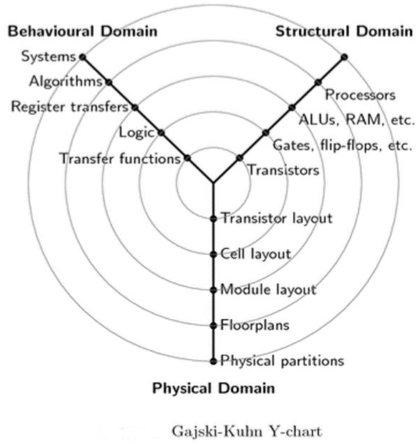
\includegraphics[width=0.45\textwidth]{imgs/ychart.jpeg}
\end{figure}

\subsection{VHDL basic concepts}
\begin{itemize}
    \item Interface
    \item Behavior
    \item Structure
    \item Testbenches
    \item Analysis
    \item Synthesis
\end{itemize}

\subsection{Modeling of behavior and structure}
\begin{itemize}
    \item Behaviour: what does the system do
    \item structure: how is the system built up of sub-modules
    \item Sub-modiles can again be described using a behavioral model or a structural model. This leads to hierarchy
\end{itemize}

\subsubsection{Example: XOR-gate}
\begin{vhdlcode}
entity xor_gate is
    port(in1, in2: in bit; out1: out bit);
end entity xor_gate;

architecture behavior of xor_gate is
begin
    out1 <= in1 xor in2;
end architecture behavior;
\end{vhdlcode}
This gives the following implementation

\begin{figure}[H]
    \centering
    \includegraphics[width=0.35\textwidth]{imgs/xor_first.png}
\end{figure}

Decomposed behavioral description:
\begin{vhdlcode}
in1 xor in2 = (in1 and in2) nor (in1 nor in2) 
\end{vhdlcode}

This can be written in VHDL as the following
\begin{vhdlcode}
architecture decomp_behavior of xor_gate is
    signal internal1, internal2: bit;
begin
    internal1 <= in1 and in2;
    internal2 <= in1 nor in2;
    out1 <= internal 1 nor internal2;
end architecture behavior;
\end{vhdlcode}

Giving the following 
\begin{figure}[H]
    \centering
    \includegraphics[width=0.75\textwidth]{imgs/xor_second.png}
\end{figure}

The and and the nor gates can then be further decomposed giving the following structural description:
\begin{figure}[H]
    \centering
    \includegraphics[width=0.75\textwidth]{imgs/xor_structure.png}
\end{figure}
Which can be described by the following VHDL

\begin{vhdlcode}
architecture structure of xor_gate is
    signal internal1, internal2: bit;
begin
    u0 : entity work.and_gate(behavior) 
        port map(in1 => in1, in2 => in2, out1 => internal1);

    u1 : entity work.nor_gate(behavior) 
        port map(in1 => in1, in2 => in2, out1 => internal2);

    u2 : entity work.xor_gate(behavior) 
        port map(in1 => internal1, in2 => internal2, out1 => out1);
end architecture structure;
\end{vhdlcode}

\subsubsection{Example of XOR-gate Testbench}
\begin{vhdlcode}
entity test_bench is
end entity test_bench;

architecture test_xor of test_bench is 
    signal in1, in2, out1 : bit;
begin
    DUT: entity work.xor_gate(structure)
        port map (in1 => in1, in2 => in2, out1 => out1);

    stimulus: process is
    begin
        in1 <= '0'; in2 <= '0'; wait for 10 ns;
        in1 <= '0'; in2 <= '1'; wait for 10 ns;
        in1 <= '1'; in2 <= '0'; wait for 10 ns;
        in1 <= '1'; in2 <= '1'; wait for 10 ns;
        wait;
    end process stimulus;
end architecture test_bench;
\end{vhdlcode}

\section{The model of time and use of delta cycles in VHDL}
\subsection{Delta-delay}
\begin{itemize}
    \item A trick used to simulate concurrent events on a sequential computer 
    \item A code line is evaluated each time something on the right-hand side is changed
    \item The resulting signal change on the left-hand side is available after a delta ($\delta$) delay
    \item If the delay is given explicitly, this delay will be used (otherwise $\delta = 1$ fs is used)
\end{itemize}

Example of specifying the delay of a gate
\begin{vhdlcode}
internal1 <= in1 and in2 after 1 ns; 
internal2 <= in1 nor in2 after 2 ns; 
out1 <= internal1 and internanternal2 after 1 ns; 
\end{vhdlcode}

\subsection{How delta-delay is used in simulation}
\begin{figure}[H]
    \centering
    \includegraphics[width=0.65\textwidth]{imgs/delta_delay.png} 
\end{figure}

\end{document}
